% !TEX root = classicthesis.tex

%************************************************
\chapter{Introduction}\label{ch:introduction}
%************************************************

Engineers have been engaged in the development of programming languages since the inception of computing. Upon establishing communication with early computers, it became evident that this interaction posed significant challenges, prompting us to seek computational assistance. It is noteworthy that, despite the remarkable advancements in contemporary computing, characterized by computers that are a million times faster and equipped with substantially increased storage capacities, the foundational principles governing programming language construction have remained relatively consistent.

While the domain explored by language designers is expansive, the avenues they have pioneered within it are relatively circumscribed. While not all programming languages follow identical trajectories, with some opting for expedient shortcuts, they tend to share fundamental commonalities. This continuity is observed across the spectrum, from Rear Admiral Grace Hopper's seminal COBOL compiler to contemporary languages that transpile into JavaScript and are often accompanied by rudimentary documentation found in a solitary, modestly edited README nestled within a Git repository.

We can analogise the ascending of a mountain to serve to illustrate the process of language implementation. It commences at the base with the program in its raw source code form, consisting solely of alphanumeric characters. Each phase in the development process involves systematic analysis and transformation, culminating in a representation at a higher conceptual level that elucidates the intended semantics—the author's instructions for the computer. Upon reaching the summit, an all-encompassing perspective of the user's program is achieved, affording a comprehensive understanding of its intended function. Subsequently, the journey descends along the opposite side of the metaphorical mountain, progressively converting the highest-level representation into successively lower-level forms, drawing closer to a format amenable to execution by the \ac{CPU}.

Let us scale through these mountain trails and introduce certain points of interest. We start with the users source code.

\section{Dissecting a Programming Language}

\subsection{Parsing}

Parsing is done by a parser, a software device that takes input text and builds a data structure called the \ac{AST}, a hierachal structure that gives a systemic representation of the input text and checking it against the lexical grammar. This is either done through top-down parsing (also known as the primordial soup approach), a method where one first looks at the highest level of the parse tree and works down the parse tree by using the rewriting rules of a formal grammar, or through bottom-up parsing, a strategy that consists of a parser starting with the input and attempting to rewrite it to the start symbol. The parser attempts to locate the most basic elements of the input, and then the elements containing these and so on. 

This process starts with lexical analysis, also known as lexing, or more informally, scanning. In this step of the implementation process, a lexer (or scanner) takes in the linear stream of code and then breaks them down into small chunks, known as tokens. There are several different types of these tokens, ranging from special characters such as \verb+;+ (known as a seperator), to string literals \verb+("Hello, World!")+ and identifiers \verb+(max)+. For example, let us consider the following expression in the C programming language:

\begin{lstlisting}[language=C++]
z = x + y * 3;\end{lstlisting}

In this expression, the lexical analysis would produce the following tokens:

\begin{lstlisting}
[(identifier, z), (operator, =), (identifier, x), (operator, +), (identifier, y), (operator, *), (literal, 3), (separator, ;)]
\end{lstlisting}

These tokens are defined by the languages lexical grammar, consisting of regular expressions and define the possible lexemes of a token. If there's a mistake when comparing with the grammar rules of the language, the parser lets the programmer know by reporting a syntax error. Note that the parsing process is standard across compilers, interpreters and translators.   

\subsection{Static Analysis}

Now, the individual characteristics of each language start coming into play. At this point, we know the syntactic structure of the code, such as the nested expressions but not much else. 

In an expression like \verb{x + y{, we know we are adding \verb+x+ and \verb+y+, but we don’t know what those names refer to. Are they local variables or global? Where are they defined? This is where we use static analysis, where we can examine programs without executing them, compared to dynamic program analysis which we perform on programs during their execution. 

The analysis process starts with binding, also known as resolution. For every identifier within the code, we find out where they are defined and connect the two together, hence defining the scope of the identifier — the region of source code where a name actually refers to a declaration. 

In a statically typed language, a language where a variable is known at compile-time instead of at run-time, this is where type checking happens. If there's an error, for example \verb+x+ and \verb+y+ are of two different types which don't support addition, a type error is reported. Note that for dynamically typed languages, such as the one we will be building, the type checking is done during runtime. 


In our metaphorical mountain, this would be the peak, where we can see the entirity of the structure and meaning of the user's program. The semantic insight from this position can be stored in several places:

\begin{itemize}
	\item Most often, it's stored right back on the syntax tree itself as an attribute, extra fields in the tree nodes that aren't initialised during the parsing process but are inserted later during compilation.
	\item It may also be stored into a symbol table, a lookup table outside of the syntax tree that contains identifiers — the names of declarations and variables. 
	\item However the most powerful method is where we transform the tree into a new data structure that directly expresses the semantics of the code. This is known as an intermediate representation. 
\end{itemize}

This is the end of what's known as the front end of the implementation process. 

\subsection{Intermediate Representations}

We can think of each stage of the compilation process as aiming to organize the data representing the user's program in a fashion that makes the next stage of the process easier to implement. The front end of the compilation process is specific to the source language of the project, while the back end if concerned with the architecture of the machine that the program will run on. This is the ``middle end'' of the compilation process. 

At this point, code is stored in a \ac{IR} that isn't tied to either the source code or the destination architecture, and acts as a bridge, or interface, between the two languages. 

This means that if we want to support multiple source languages and target platforms we don't need to write multiple compilers for each possible combination of language and architecture, but instead, using a shared intermediate representation, we write one front end for each source langauge and one back end for each target architecture. This means we can mix and match, drastically reducing development time. However, this isn't the only reason we'd like to use a intermediate representation.

\subsection{Optimization}

Once we have a semantic overview of the user's program, we can substitute it with a different program that performs the same operations, just more efficiently, optimizing it. 

One form of this is constant folding; if one expression always evaluates to the same value (e.g it is constant) we can evaluate the expression at compile time and replace the code calculating the constant with the resulting number. If the original program was this:

\begin{lstlisting}[language=C++]
footballVolume = 4/3 * 3.14159 * (1)^3;
\end{lstlisting}

We could calculate this in the compiler and replace the code with:

\begin{lstlisting}[language=C++]
footballVolume = 4.18878667;
\end{lstlisting}

Another method is known as strength reducation, where expensive operations are replaced with equivalent but less expensive operations. Consider the following C code snippet: 

\begin{lstlisting}[language=C]
int i, sum = 0;
for (i = 1; i <= n; ++i) {
  sum += i;
}
printf("sum: %d\n", sum);

\end{lstlisting}

Assuming no arithmetic overflow, we can rewrite the code to be:

\begin{lstlisting}[language=C]
int sum = n * (1 + n) / 2;
printf("sum: %d\n", sum);
\end{lstlisting}

This makes use of the following mathematical standard summation for consecutive natural numbers: 
\begin{equation}\sum_{n=1}^i n = \frac{1}{2}n(n+1)\end{equation}
This same method of choosing more computationally efficient algorithms for performing operations is the key to strength reducation. However, note that the ``optimized'' version might actually be slower than the original version if \verb+n+ were sufficiently small and the particular hardware happens to be much faster at performing addition and looping operations than multiplication and division.

Furthermore, while the term ``optimization'' shares its root with ``optimal'', it is uncommon for the optimization process to yield a system that is genuinely optimal in all respects. Typically, a system can be optimized, not in an absolute sense, but rather in relation to a specific quality metric, which may conflict with other potential metrics. Consequently, the optimized system usually achieves optimality only within a particular application or for a specific target audience.

For instance, one might choose to reduce the execution time of a program, even if it results in increased memory consumption. In situations where conserving memory space is critical, deliberately opting for a slower algorithm may be a preferable trade-off. Frequently, there is no universally ideal design that can excel in all scenarios. Engineers must make calculated trade-offs to optimize the attributes that are most relevant to the task at hand. Several programming languages, such as CPython and Lua generate relatively unoptimized code and in exchange focus on performance effort during the runtime. 

\subsection{Code Generation}

After optimizing the user's source code, we move to coverting into machine code, a form that the machine can actually run. This is known as the generating code, where the code that is generated is usually some permutation of assembly code. 

Although somewhat unrelated, we should mention that when code generation takes place at runtime, such as in \ac{JIT} compilation, it is important that the process is efficient with respect to space and time. Despite its generally generating less efficient code, \ac{JIT} code generation can take advantage of profiling information that is available only at runtime.

This is the end of the middle end of the compilation process, and now part of the back end, the downward descent down our metaphorical mountain. We have gained an understanding of the user's program and now devolve the code, each step of the back end making the code more and more primitive so a simple \ac{CPU} can execute it. 

We can either produce instructions for a real \ac{CPU} or a virtual one. If we generate machine code for a real \ac{CPU} we are given an executeable that is loaded and executed directly on the chip by the machine's operating system. This results in fast code, but the generating process is significantly long due to complex pipelines, and a large and complicated instruction set. 
 
Furthermore, the produced executeable is also tied to the machine's architecture, say x86 or ARM, resulting in a lack of portability. To circumvent this, we can have our compiler produce virtual machine code, code that runs for some hypothetical machine. This is known as bytecode, since each instruction is often just a single byte long.

This synthetic set of instructions are designed to be based more around the properties of the source language rather than the the quirks of a computer architecture, sort of like a dense, binary encoding of the language’s low-level operations. 

\subsection{Virtual Machine}

However, this virtual code is useless without a chip that can understand it. We have two options, the first being a  `mini-compiler' for each real architecture we want out program to run to that converts the bytecode to native machine code for that language. This may seem counterproductive since we are trying to circumvent the architecture roadblock, but this step is relatively simple, and we able to retain the rest of the compiler across the machines we wish to support, meaning the bytecode essentially functions as a intermediate representation.

The other option would be a \ac{VM}, a program that emulates our hypothetical chip and supporting out virtual architecture at runtime. This implementation is slower than the prior method since every instruction must be simulated at runtime before executing, however in exchange a \ac{VM} offers simplicity and portability. 

There are two main types of virtual machines, system virtual machines (also known as full virtualisation \acsp{VM}) and process virtual machines. System virtual machines are a complete substitute for a real machine, provdiing the functionality to execute entire operating systems, while process virtual machines are designed to execute certain program in an isolated enviroment. This is the type we will be using throughout the project. 

\subsection{Runtime} 

We are finally at the end of the process of moulding the user's program into a form that we can run. The last step is running it. If we had compiled it to real machine code we would just tell the operating system to load and run the executeable file that is generated, however with bytecode we need to start the virtual machine and load the program through that. 

The runtime, often referred to as the runtime environment, is a crucial component in most programming languages, except for the most basic low-level ones. It provides essential services during program execution. One such service is memory management automation, which necessitates the presence of a garbage collector to reclaim unused memory.

Additionally, if the language supports ``instance of'' tests to determine object types, a mechanism for tracking the type of each object during runtime is required. The integration of these services into a program depends on the language's nature.

In the case of fully compiled languages, the code responsible for the runtime is directly inserted into the resulting executable. For example, in Go, each compiled application includes its own copy of Go's runtime, embedded within it. Conversely, languages that run within interpreters or virtual machines have the runtime environment residing in those environments. This operational model is commonly employed in languages like Java, Python, and JavaScript.

\section{Alternative Methods and Shortcuts}

This comprehensive journey covers every conceivable phase of implementation, and many languages do indeed traverse this entire route. However, there are a few  shortcuts and alternative paths available.

\subsection{Single-Pass Compilers}

A single-pass compiler, also known as a one-pass compiler is a compiler that passes through each compilation unit, such as a source file, only once and immediately transforms this into the final machine code that will be run. This means it skips the intermediate representation phase, does not allocate a syntax tree and does not reprocess the compilation unit in each sequential pass. In theory, this produces a smaller and faster processor, but compiler optimization is highly limited due to the limited scope of information available. Furthermore, many effective forms of compiler optimization, such as strength reduction, require multiple passes over structures such as a nested loop. 

\subsection{Tree-Walk Interpreters}

This approach functions by executing code right after it is parsed to an AST or using it to generate native code just-in-time. This is done by the interpreter traversing the syntax tree one branch at a time, evaluating each node as it parses. This again means each sentence only needs to be parsed once, and the \ac{AST} keeps the global program structure and relations (which is lost in bytecode representation). However, an \ac{AST} causes large overhead from visitng the tree (a less sequential representation causes traversal of more pointers) and because syntax nodes are useless during the process.

\subsection{Transpilers}

Creating a complete back end for a language is often a substantial undertaking. If we happen to possess a pre-existing, generic intermediate representation as our target, we can seamlessly integrate our front end with it. However, in cases where this isn't an option, we may find ourselves facing a daunting challenge.

Here's an alternative approach to consider: Instead of expending significant effort in the back end to transform the semantics into a lower-level target language, we can generate a string of valid source code for another language that shares a similar high-level nature with our own (compared to a traditional compiler which translates from high level to low level). This opens up the possibility of utilizing the existing compilation tools for that language to facilitate the transition from our elevated position to an executable form.

This methodology was once referred to as a ``source-to-source compiler'' or ``transcompiler.'' With the emergence of languages that compile to JavaScript for browser-based execution, it has gained a certain trendy reputation and is commonly known as a ``transpiler'' among the more hip programming circles.

\begin{figure}[h]
\centering
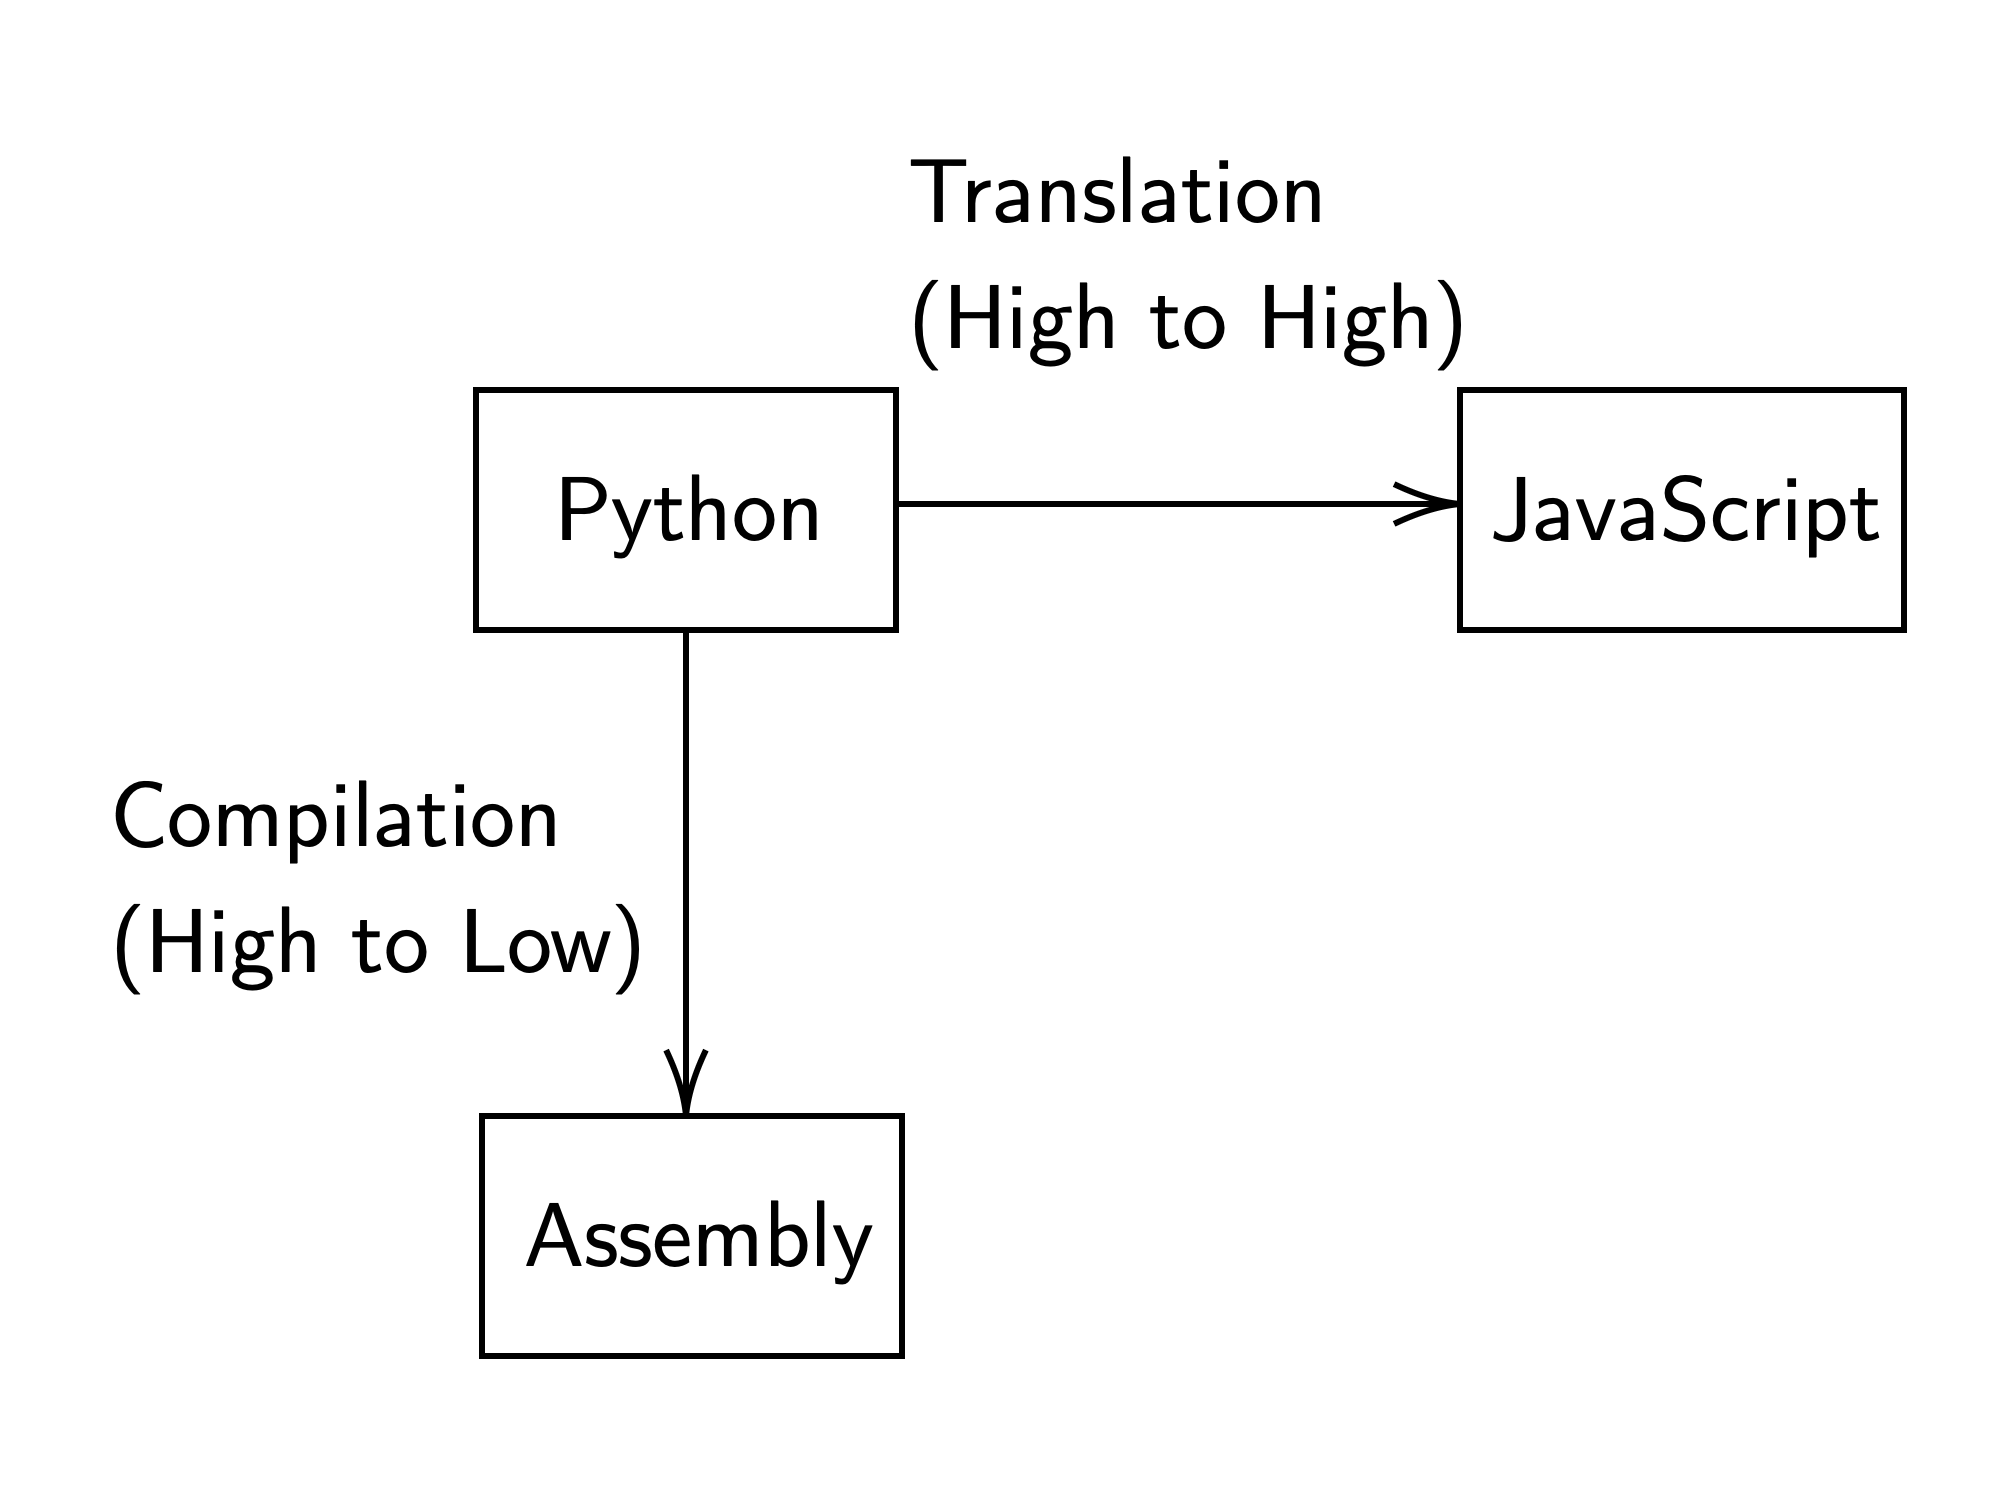
\includegraphics[width=0.75\textwidth]{gfx/transpiler.png}
\caption{Transpilers}
\end{figure}

Another valuable application of source-to-source compiling involves the translation of legacy code to adapt it to the next iteration of the underlying programming language or an \ac{API} that introduces changes, potentially breaking backward compatibility. This process also includes automatic code refactoring, which is useful when programs are impractically large or time-consuming to be done by hand. 

The parser of a transpiler is identical to other compilers, and analysis may be skipped if the source language is similar to the target language, meaning the corresponding syntax is output to the intended language straight after parsing. 

However, if the two language are not as syntactically similar, semantic analysis will be conducted, possibly with compiler optimizations as well, analogous to a full compiler. The difference comes at code generation, where instead of resulting in machine code, or some other binary language, we are produced with the program in the desired language which we can then run through that languages compilation process. 

\subsection{Just-In-Time Compilation}

This approach is more risky than those above, and involves compiling once the program is loaded at run-time on the user's machine, natively for the architecture of the end machine. This means you we can then compile for a machine architecture which was originally unknown and furtheremore at high speed. Although it is possible to compile the source code to machine code at run-time, often it is bytecode that is translated. 

This is actually a combination of two previous approaches in translation to machine code, \ac{AOT} compilation and interpretation, and \ac{JIT} tries to combine the advantges of both, albeit with some of the drawbacks. This compilation process results in speeds similar to pre-compiled code and flexibility comparitive to interpretation, hence it's use in dynamically typed languages. The overhead of this process however is a combination of the methods it draws upon, compiling and linking (not just interpreting)

At the highest levels \acsp{JIT} insert profiling hooks to understand which areas of the programs are most performance critical and over time recompile those with greater and more advanced optimizations. 

\section{Compilers and Interpreters}

We would like to start by defining a clear line between compilers and interpreters, which so far have almost been used interchangeably. In theory, a programming language can have both a compiler and interpreter, but in practice it often just implements just one. 

\subsection{Compilers}

To distinguish compilers from interpreters, it's crucial to understand that compilers are primarily concerned with translating source code into another form, typically a lower-level representation or machine code. This transformation allows for efficient execution of the program in the target environment. For example, when a high-level programming language like C++ is compiled, the source code is translated into machine code, and the result is an executable file. Importantly, the compilation process \textbf{does not} involve the direct execution of the program; instead, it produces an independent executable that can be run later. Consequently, once the compilation is complete, the original source code is no longer required to execute the program, making it suitable for distribution and deployment on various systems, as well as a greater security factor for preventing modification of the source code. This separation of compilation and execution is a key characteristic of compilers, as they focus on generating efficient stand-alone executables.

\subsection{Interpreters}

In contrast to compilers, interpreters operate by directly executing the source code ``on the fly''. When a programming language is implemented with an interpreter, it takes the source code as input and immediately begins executing it. This approach is often described as ``running from source'' because there is no intermediate step of generating a separate executable file. Instead, the interpreter interprets and executes each line or statement of the source code in real-time. This immediate execution can be advantageous for tasks like debugging, as errors are reported as they occur in the source code. However, it can also be less efficient than compiled code since the interpreter must repeatedly analyze and execute the code line by line. Interpreters are commonly used in scripting languages like Python and JavaScript, where rapid development and platform independence are more critical than raw execution speed.

An example of a language utilizing both implementations is CPython, which from the users perspective seems like as an interpreter — they can clearly see the program run from source. However, under the hood the code is parsed and converted into an internal bytecode format, which is then executed within the \ac{VM}, which is compiler like. We illustrate some other lagnuages and whether they use a compiler, interpreter or both:

\begin{figure}[h]
\centering
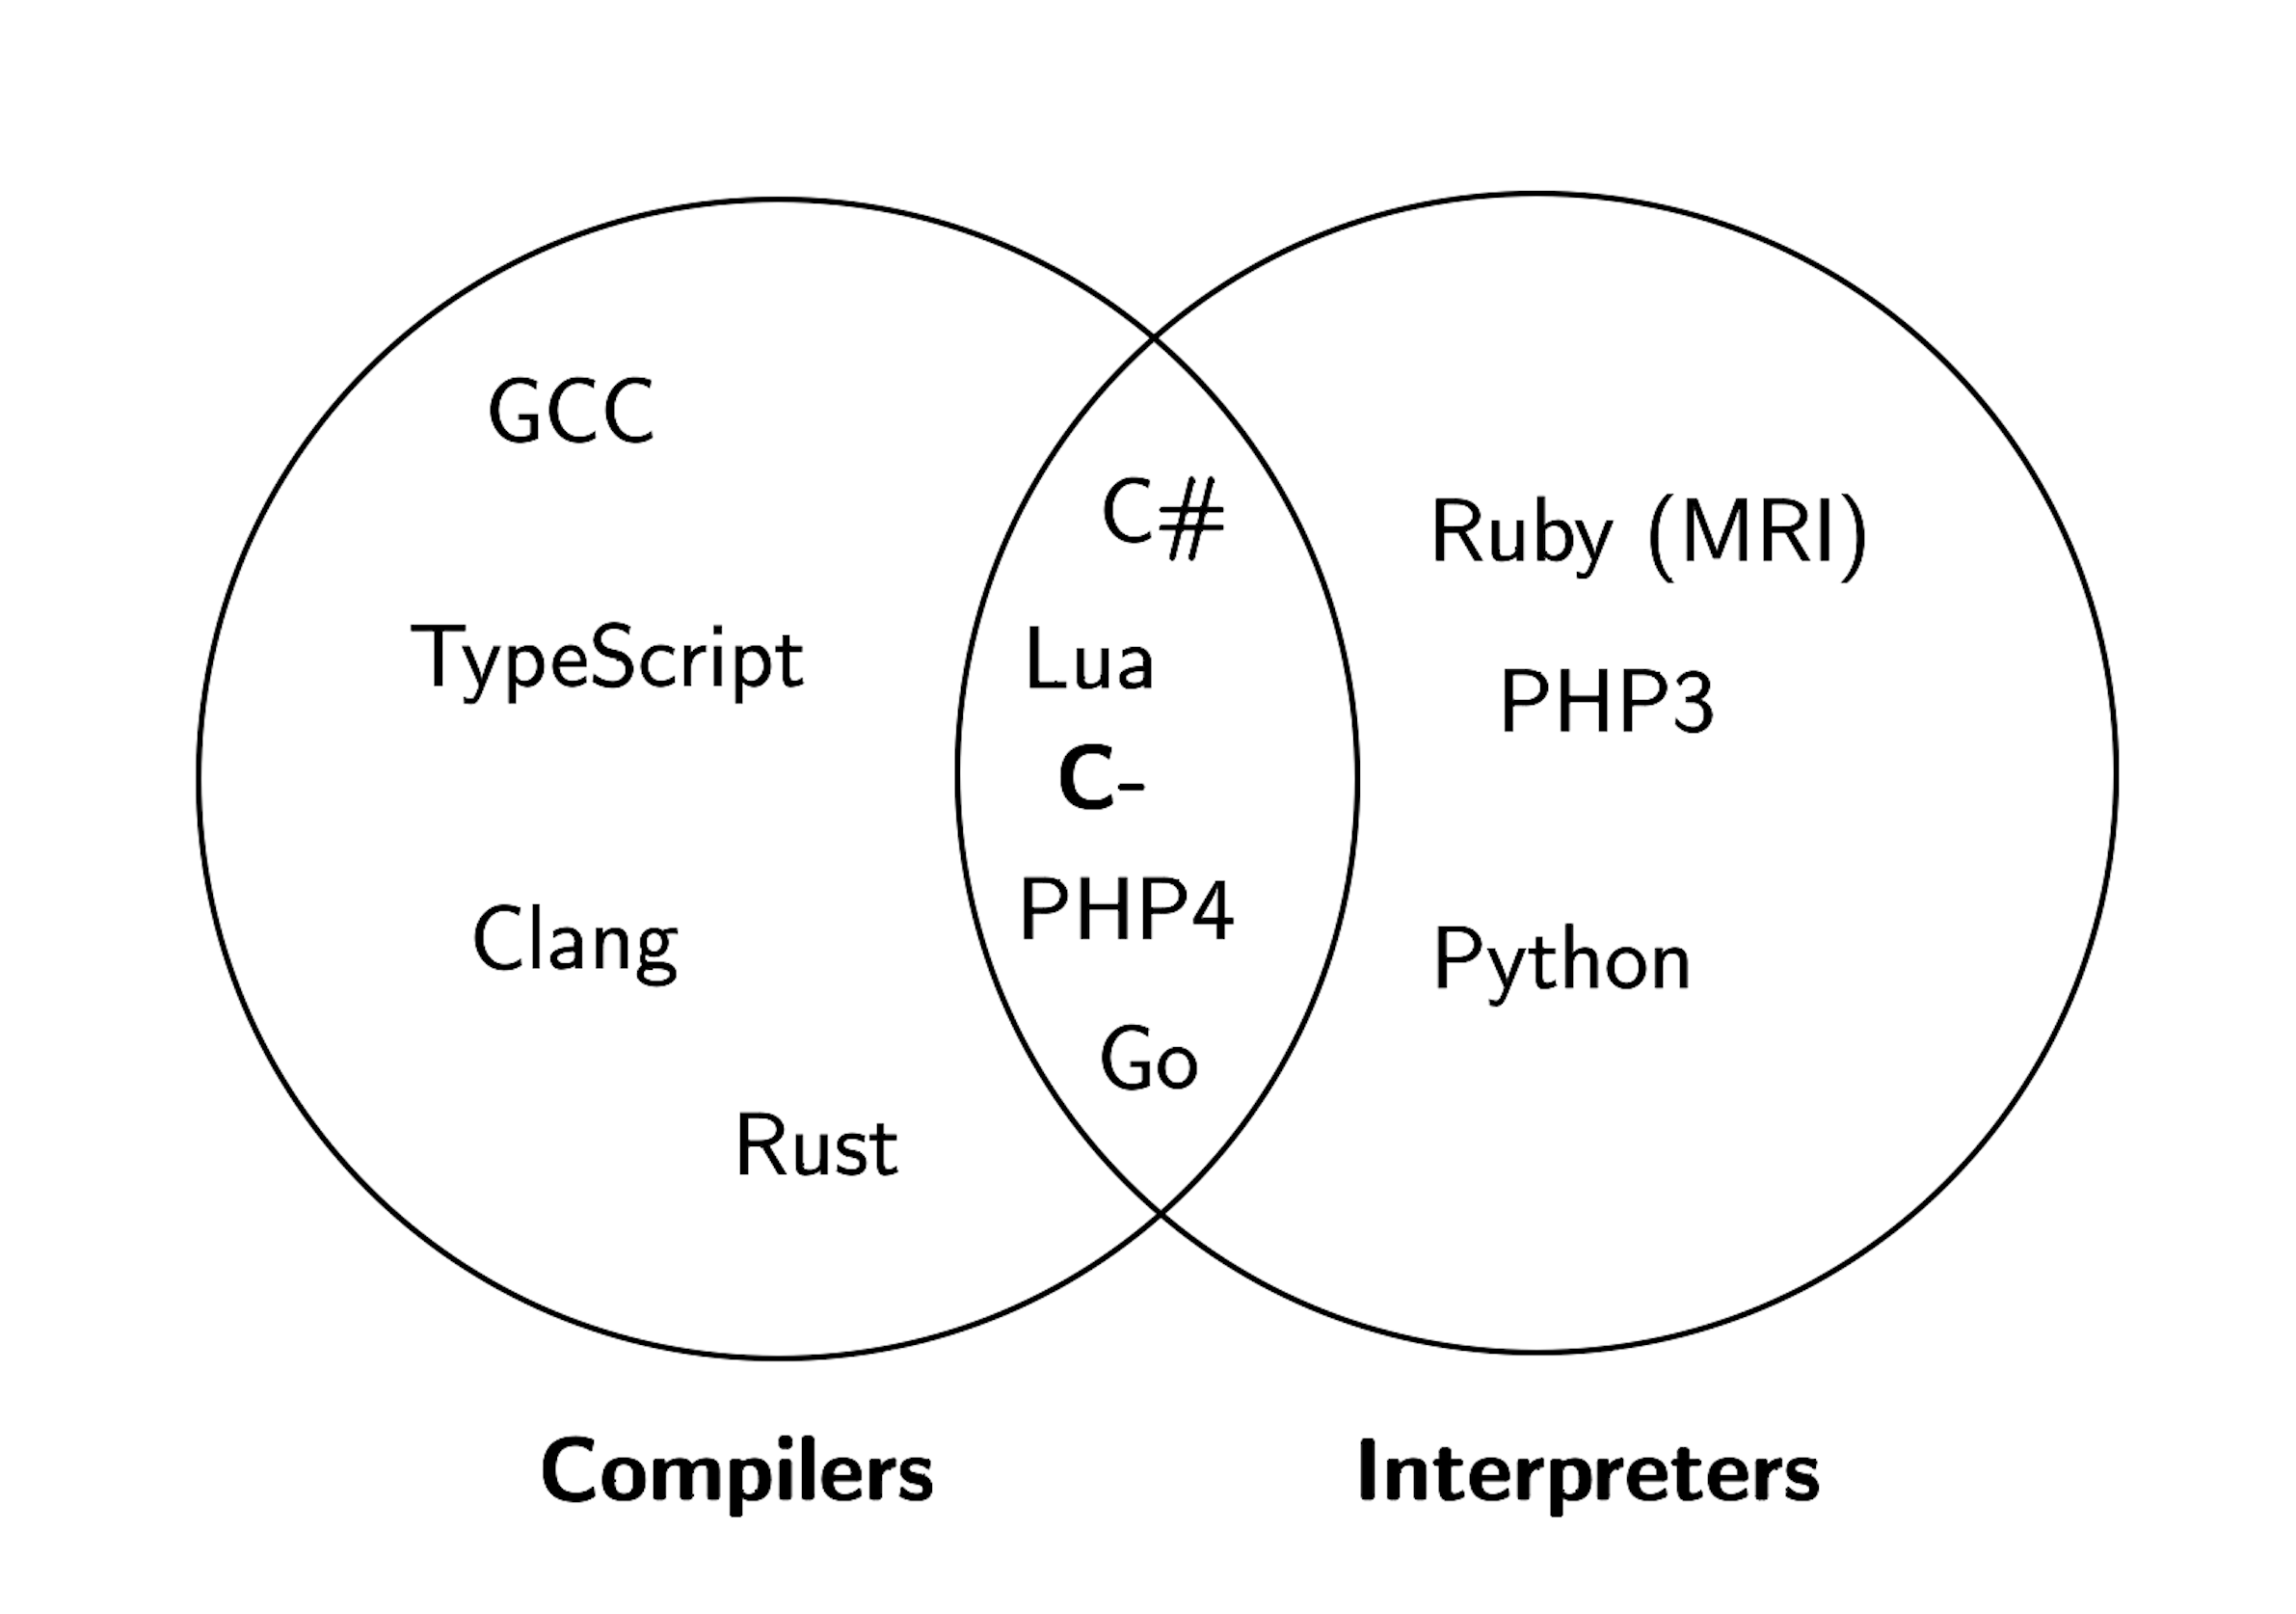
\includegraphics[width=0.75\textwidth]{gfx/venn.png}
\end{figure}

Our implementation, C-, lives in the middle area as it internally compiles to bytecode and then sends it to the \ac{VM}. 





%*****************************************
%*****************************************
%*****************************************
%*****************************************
%*****************************************




